
\section{¿Qué es un modelo neuronal?}

En esta sección, se explica qué es un modelo neuronal, sus características y cómo funciona en el contexto de la inteligencia artificial. 

Los modelos neuronales son estructuras computacionales inspiradas en el cerebro humano, diseñadas para procesar información mediante una red de unidades interconectadas que imitan, de manera simplificada, la forma en que las neuronas biológicas se comunican entre sí cite{goodfellow2016deep}.

Los descurbrimientos del Premio Nobel de biología español, Santiago Ramón y Cajal sobre la estructura y funcionamiento de las neuronas, proporcionaron las bases para la comprensión del sistema nervioso en el que se basan los modelos de inteligencia artificial. A finales del siglo XIX, Cajal formuló la teoría de que las neuronas son células individuales conectadas por sinapsis, una idea que revolucionó la neurociencia y sirvió de inspiración para los modelos computacionales de redes neuronales. Su trabajo permitió comprender cómo las señales eléctricas viajan entre las neuronas y cómo se pueden formar conexiones adaptativas, conceptos que más tarde serían adoptados en el diseño de redes neuronales artificiales.

Un modelo neuronal es una arquitectura matemática que busca resolver problemas complejos de aprendizaje mediante el procesamiento de datos. Está compuesto por una serie de unidades de procesamiento, conocidas como neuronas artificiales, organizadas en capas. Cada capa recibe la salida de la capa anterior, aplica una función matemática sobre los datos y transmite el resultado a la siguiente capa. Este proceso se repite de manera secuencial hasta que se alcanza la capa de salida, que proporciona el resultado final del modelo \cite{bishop2006pattern}.

\begin{figure}[H]
    \centering
    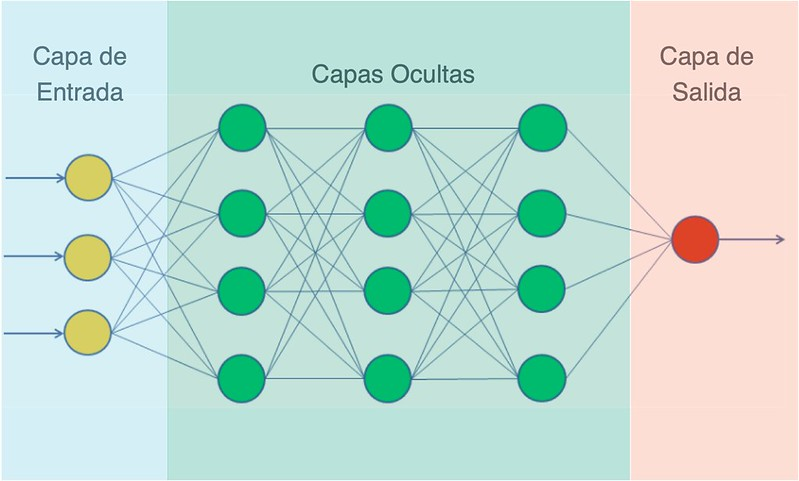
\includegraphics[width=0.8\textwidth]{./img/modelo/capas.png}
    \caption{Esquema de redes neuronales. \cite{aprendeia2021deep}}
    \label{fig:esq-capas}
\end{figure}

Las neuronas dentro de un modelo neuronal no operan de forma aislada, sino que están conectadas entre sí a través de enlaces denominados "pesos". Estos pesos determinan la importancia de la señal que se transmite de una neurona a otra. Durante el proceso de entrenamiento, los pesos se ajustan con el objetivo de minimizar el error en la salida del modelo, lo que permite que el modelo "aprenda" de los datos y mejore su capacidad para predecir o clasificar nueva información \cite{haykin2009neural}.

El proceso de entrenamiento de un modelo neuronal implica la retroalimentación o backpropagation, donde el error de la predicción se calcula y se distribuye hacia atrás a través de la red para ajustar los pesos de manera que el modelo se optimice progresivamente. En este sentido, el modelo neuronal tiene la capacidad de adaptarse a distintos tipos de datos y mejorar su rendimiento con el tiempo \cite{nielsen2015neural}.

A grandes rasgos, un modelo neuronal es una estructura computacional que imita el funcionamiento del cerebro humano para procesar y aprender de datos, y se utiliza en tareas como clasificación, predicción y reconocimiento de patrones.


\subsection{¿Qué tipos de modelos neuronales existen?}

En esta sección se explican cuales son tipos de modelos neuronales existen y sus características principales. 

Los modelos neuronales pueden clasificarse según su estructura, la forma en que procesan la información y la aplicación específica a la que están destinados. Estos modelos neuronales son fundamentales para resolver una variedad de problemas en áreas relacionadas con la inteligencia artificial como la visión por computadora, el procesamiento del lenguaje natural y el reconocimiento de patrones.

Uno de los tipos más comunes de modelos neuronales es el perceptrón multicapa (MLP), que está formado por varias capas de neuronas organizadas en una estructura jerárquica. Cada capa en un MLP recibe la salida de la capa anterior y la procesa mediante una función de activación antes de pasar el resultado a la siguiente capa. Este tipo de red se utiliza principalmente para tareas de clasificación y regresión, y su entrenamiento se realiza utilizando algoritmos como el de retropropagación. Es el tipo de modelo que se utiliza en este proyecto para obtener un modelo capaz de detectar instrusiones en una red informática. \cite{goodfellow2016deep}

Otro tipo importante de modelo neuronal es la red neuronal convolucional (CNN), que está diseñada específicamente para procesar datos con una estructura de cuadricula, como las imágenes. En una CNN, las neuronas están organizadas en capas convolucionales que aplican filtros a los datos de entrada para extraer características relevantes, como bordes, texturas o formas. Esta estructura permite que las CNN sean altamente eficaces para tareas como el reconocimiento de imágenes y la visión por computadora \cite{goodfellow2016deep}.


\begin{figure}[H]
    \centering
    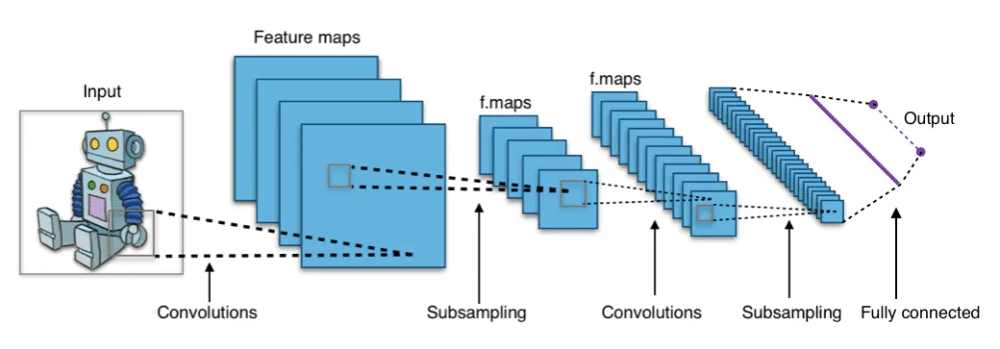
\includegraphics[width=0.8\textwidth]{./img/modelo/CNN.png}
    \caption{Esquema de redes neuronal convolucional. \cite{uniteai2020cnn}}
    \label{fig:esq-CNN}
\end{figure}


Las redes neuronales recurrentes (RNN), por otro lado, son adecuadas para procesar secuencias de datos, como el texto o el audio. Las RNN son únicas porque sus neuronas tienen conexiones que permiten que la información fluya hacia atrás a lo largo del tiempo, lo que las hace útiles para modelar dependencias temporales en los datos. Este tipo de red es comúnmente utilizado en tareas de procesamiento de lenguaje natural y en modelos de predicción de series temporales \cite{haykin2009neural}.

En un enfoque más avanzado, existen las redes generativas antagónicas (GAN), que se componen de dos redes neuronales: un generador y un discriminador. El generador crea datos falsos a partir de ruido, mientras que el discriminador intenta diferenciar entre los datos reales y los generados. A través de un proceso de entrenamiento competitivo, ambas redes mejoran en sus respectivas tareas. Las GANs se utilizan principalmente en la generación de imágenes, música y otros tipos de contenido artístico \cite{nielsen2015neural}.

\subsection{Función de perdida}
En esta sección se explica que es una función de pérdida y su importancia en el proceso de entrenamiento de un modelo neuronal. También se justifica el uso de las funciones de pérdida que se emplean para el entrenamiento de los modelos de este trabajo.

Una función de pérdida es un componente fundamental en el entrenamiento de modelos de aprendizaje automático, cuya finalidad consiste en cuantificar la discrepancia entre las predicciones generadas por el modelo y los valores reales esperados. Esta medida permite guiar el proceso de optimización, ya que el objetivo durante el entrenamiento es minimizar dicha pérdida para mejorar la precisión del modelo.\cite{eitca_loss_function}

Las funciones de pérdida desempeñan un papel central en la formulación matemática del aprendizaje supervisado, al establecer una métrica que penaliza el error cometido por el modelo. Esta penalización permite que los algoritmos de optimización, como el descenso por gradiente, ajusten iterativamente los parámetros del modelo en la dirección que reduce la pérdida total. Para que esta estrategia sea efectiva, la función de pérdida debe poseer ciertas propiedades fundamentales:

\begin{itemize}

    \item\textbf{Diferenciabilidad}: Permite el cálculo de gradientes necesarios para optimizar los parámetros mediante técnicas basadas en derivadas, como el descenso por gradiente.

    \item\textbf{Convexidad (deseable)}: Favorece la convergencia hacia un mínimo global, aunque en la práctica, muchos modelos no lineales presentan funciones de pérdida no convexas.

    \item\textbf{Estabilidad numérica}: Previene errores computacionales al manejar valores extremos o transformaciones exponenciales, manteniendo precisión durante el entrenamiento.

 	\item\textbf{Sensibilidad al error}: Garantiza que los errores mayores se penalicen de forma más significativa, orientando el modelo hacia mejores predicciones.

	\item\textbf{Escalabilidad}: Permite su aplicación eficiente en contextos con grandes volúmenes de datos y arquitecturas de red complejas.

\end{itemize}

Estas propiedades aseguran que la función de pérdida cumpla su objetivo central, actuar como un mecanismo confiable y eficiente para guiar la actualización de los parámetros del modelo. \cite{ultralytics_loss_function}

En el caso específico del modelo de clasificación binaria, se opta por la función BCEWithLogitsLoss (Binary Cross Entropy with Logits Loss), que está especialmente recomendada para utilizarse en entornos de aprendizaje profundo como PyTorch, entorno utilizado en el desarrollo práctico de este proyecto. Esta función combina en una sola operación dos pasos fundamentales: la aplicación de la función sigmoide y el cálculo de la entropía cruzada binaria. Al integrar ambos procedimientos en una única función, se obtienen varias ventajas prácticas.\cite{datacamp_loss_function}

En primer lugar, se mejora la estabilidad numérica, ya que evita operaciones redundantes que podrían dar lugar a pérdidas de precisión, especialmente al manejar las salidas no normalizadas del modelo (logits) con valores extremos.

En segundo lugar, se optimiza el rendimiento computacional, al reducir el número de transformaciones necesarias antes del cálculo de la pérdida. 

Finalmente, permite trabajar directamente con logits, lo cual simplifica la implementación y reduce errores potenciales derivados de transformaciones incorrectas. \cite{bigdatafran_pytorch_classification}




\subsection{Algoritmo de optimización}\label{sec:alg-opt}
En esta sección se explica qué es un algoritmos de optimización,su funcionamiento, sus principales características, su importancia dentro del proceso de entrenamiento de modelos neuronales y algunos ejemplo de los algoritmos de optimización más utilizados.

Un algoritmo de optimización es un conjunto de procedimientos matemáticos y computacionales cuyo propósito es encontrar el mejor valor posible (o el más cercano a este) para un conjunto de parámetros o variables dentro de un problema específico. Estos algoritmos buscan minimizar o maximizar una función objetivo, que representa el rendimiento del sistema o modelo a optimizar. En el contexto de entrenamiento de redes neuronales, la función objetivo comúnmente se refiere a una función de pérdida, que cuantifica la diferencia entre las predicciones del modelo y las etiquetas reales de los datos. Los algoritmos de optimización ajustan los parámetros (pesos y sesgos) de la red neuronal durante el proceso de entrenamiento con el fin de reducir dicha diferencia \cite{goodfellow2016deep}.


El funcionamiento de un algoritmo de optimización se basa en un proceso iterativo en el que se ajustan los parámetros de la red neuronal utilizando información acerca del gradiente de la función de pérdida con respecto a estos parámetros. En este contexto, la retropropagación juega un papel crucial, ya que es el método utilizado para calcular esos gradientes. A través de la retropropagación, el error de la red se propaga hacia atrás desde la capa de salida hasta las capas anteriores, permitiendo calcular cómo cada parámetro contribuye al error total. Posteriormente, el algoritmo de optimización utiliza estos gradientes calculados por la retropropagación para actualizar los parámetros de la red en la dirección opuesta al gradiente, con el objetivo de reducir progresivamente la pérdida. Generalmente, se utilizan técnicas de descenso de gradiente para realizar estos ajustes. Durante cada iteración, el algoritmo calcula el gradiente de la función de pérdida a través de la retropropagación y lo utiliza para modificar los parámetros de manera eficiente, buscando alcanzar el mínimo global o local de la función de pérdida \cite{bottou2010large}.

\begin{figure}[H]
    \centering
    \includegraphics[width=0.8\textwidth]{./img/modelo/retropropagacion.png}
    \caption{Esquema de algoritmo de optimización usando los gradiente calculados por la retropropagación. \cite{msmk2023backpropagation}}
    \label{fig:esq-Optimizacion}
\end{figure}



Las características clave de los algoritmos de optimización incluyen la tasa de aprendizaje, la capacidad para escapar de mínimos locales, y la convergencia en un tiempo razonable. La tasa de aprendizaje (learning rate o lr) es un hiperparámetro crítico que determina la magnitud de los ajustes que se realizan en los parámetros del modelo durante cada iteración. Si el learning rate es muy alto, el algoritmo puede saltar el mínimo global, por otro lado, si es muy baja, el proceso puede volverse muy lento. Los métodos de optimización varían en cuanto a la forma en que gestionan estas características, algunos métodos mejoran la eficiencia utilizando técnicas como el momento, la normalización del gradiente, o el uso de segunda orden \cite{kingma2014adam}.


La importancia de los algoritmos de optimización en el entrenamiento de redes neuronales es fundamental, ya que la capacidad de un modelo para aprender de los datos y generalizar de manera efectiva depende en gran medida de cómo se optimizan los parámetros de la red. Un algoritmo de optimización bien elegido y configurado puede significar la diferencia entre un modelo con un rendimiento subóptimo y uno que logra altos niveles de precisión y eficiencia. De esta manera, la correcta selección y ajuste de estos algoritmos se considera un aspecto crucial para el desarrollo exitoso de modelos de aprendizaje profundo y redes neuronales \cite{goodfellow2016deep}.

Existen varios algoritmos de optimización ampliamente utilizados en el entrenamiento de redes neuronales. Entre los más comunes se encuentran el Descenso de Gradiente Estocástico (SGD), Momentum, Adagrad, RMSprop y Adam. El SGD es uno de los más simples y fundacionales, pero sufre de inestabilidad debido a su naturaleza estocástica y la falta de adaptación de la tasa de aprendizaje. Momentum ayuda a mejorar la convergencia al incorporar la información de los gradientes pasados, lo que permite que el modelo escape de los mínimos locales más fácilmente. Adagrad adapta la tasa de aprendizaje para cada parámetro, mientras que RMSprop ajusta la tasa de aprendizaje utilizando una media móvil del gradiente, lo que mejora la estabilidad \cite{bottou2010large}.

Sin embargo, el algoritmo más recomendado para entrenar un modelo de clasificación binaria es Adam (Adaptive Moment Estimation). Adam combina las ventajas del descenso de gradiente estocástico y el momento, adaptando la tasa de aprendizaje de manera eficiente para cada parámetro del modelo. Esto lo hace particularmente adecuado para tareas de clasificación binaria, ya que garantiza una convergencia más rápida y estable, minimizando el riesgo de sobreajuste (overfitting) mientras se optimizan los parámetros del modelo. Sin embargo, una variante reciente de Adam, conocida como AdamW, introduce un cambio importante en la forma en que se maneja la regularización de los parámetros. AdamW separa explícitamente la actualización de los pesos y la regularización (típicamente L2 o weight decay), lo que mejora la eficacia de la regularización sin interferir con la adaptación de la tasa de aprendizaje.

Aunque ambos algoritmos, Adam y AdamW, tienen un rendimiento destacado en tareas de clasificación binaria, AdamW se ha demostrado más eficaz en la prevención de sobreajuste en redes neuronales complejas. Esto se debe a su tratamiento explícito del weight decay, lo que permite una mejor generalización en problemas con grandes volúmenes de datos como el que se trata en este proyecto. Sin embargo, Adam sigue siendo una opción popular y efectiva, especialmente cuando se trabaja con redes neuronales menos complejas o cuando se desea una mayor estabilidad y rapidez de convergencia. En general, AdamW es preferido en situaciones donde la regularización adecuada es crucial, pero Adam sigue siendo una opción sólida y eficiente. \cite{kingma2014adam}.


\section{Parámetros e hiperparámetros}
En este apartado se explica que son los parámetros y los hiperparámetros de un modelo neurnal. También se listan y describen los principales hiperparámetros que se deben de tener en cuenta al entrenar un modelo neuronal. 

Los parámetros de un modelo neuronal son los valores ajustables que el modelo aprende a partir de los datos durante el proceso de entrenamiento. Estos parámetros incluyen los pesos y sesgos de las conexiones entre las neuronas de las diferentes capas de la red neuronal. Los pesos determinan la importancia de las entradas de cada neurona, mientras que los sesgos permiten ajustar la salida de cada neurona antes de la activación. Como se explica en los apartado anteriores, el aprendizaje de estos parámetros se realiza mediante algoritmos de optimización como el gradiente descendente, los cuales buscan minimizar la función de pérdida. \cite{goodfellow2016deep}


Los hiperparámetros son los valores que se configuran antes del entrenamiento y no se ajustan directamente durante el proceso de aprendizaje. Este tipo de parámetros controlan el comportamiento del proceso de entrenamiento y afectan la capacidad del modelo para aprender patrones complejos de los datos. A diferencia de los parámetros, los hiperparámetros deben ser establecidos manualmente o mediante técnicas de optimización específicas, como la búsqueda en cuadrícula o la búsqueda aleatoria, técnicas que se aplcian en las siguientes secciones de este documento. Los hiperparámetros influyen en aspectos clave como la velocidad de aprendizaje, la regularización y la estructura de la red \cite{chollet2018deep}. Los más importantes son:

\begin{itemize}

    \item \textbf{Tasa de aprendizaje (Learning rate)}: Controla la magnitud de los ajustes realizados en los pesos durante cada iteración del entrenamiento. Como se comenta en \ref{sec:alg-opt} \nameref{sec:alg-opt}, una tasa demasiado alta puede hacer que el modelo no converja, mientras que una tasa demasiado baja puede llevar a una convergencia muy lenta.
    
    \item \textbf{Número de épocas (Epochs)}: El número de épocas se refiere a cuántas veces el algoritmo de entrenamiento recorre todo el conjunto de datos. Un número adecuado de épocas permite que el modelo aprenda de manera efectiva, sin embargo, demasiadas épocas pueden llevar al sobreajuste.
    
    \item \textbf{Tamaño del lote (Batch size)}: El tamaño del lote determina la cantidad de ejemplos utilizados en cada actualización de los pesos. Un tamaño de lote pequeño puede hacer que el modelo sea más ruidoso y difícil de entrenar, mientras que un tamaño de lote grande puede hacer que el entrenamiento sea más estable, pero menos eficiente.
    
    \item \textbf{Número de capas ocultas (Hidden layers)}: Este hiperparámetro define la profundidad de la red neuronal, es decir, el número de capas intermedias entre la capa de entrada y la capa de salida. Un mayor número de capas permite modelar funciones más complejas, pero también aumenta el riesgo de sobreajuste.
    
    \item \textbf{Número de neuronas por capa (Hidden factor)}: Este parámetro establece la cantidad de neuronas en cada capa oculta. Un mayor número de neuronas puede mejorar la capacidad del modelo para capturar patrones complejos, aunque también aumenta el tiempo de entrenamiento y la complejidad computacional.
\end{itemize}



\section{Modelo neuronal de clasificación binaria}
En esta sección se describe el proposito y los procedimientos empleados para el desarrollo del modelo de clasificación binaria. Se detalla el proceso de selección de hiperparámetros, así como las distintas arquitecturas diseñadas con el fin de identificar la combinación que optimiza el rendimiento del modelo. Además, se presenta una comparación entre las arquitecturas evaluadas para determinar la más adecuada.

%Finalmente, se especifican las métricas utilizadas para la evaluación y selección de las mejores combinaciones de hiperparámetros.

\subsection{Proposito del modelo de clasificación binaria}
El modelo de clasificación binaria se ha diseñado con el obtejivo de identificar de manera precisa y eficiente si una instancia de tráfico de red corresponde a una actividad legítima o a un comportamiento malicioso. Su función principal consiste en distinguir entre accesos normales y posibles intentos de intrusión, permitiendo así la detección temprana de ataques y contribuyendo a la protección proactiva de los sistemas informáticos.

\subsection{Diseño del modelo e hiperparámetros seleccionados}

El modelo de clasificación binaria se ha diseñado para utilizar 



Los hiperparámetros que han sido seleccionados para encontrar la mejor configuración para el modelo de clasificación binaria diseñado son: el batch size, la tasa de aprendizaje (learning rate) y el número de épocas. Estos hiperparámetros resultan imprescindibles en el entrenamiento de modelos de clasificación binaria, dado que influyen directamente en la eficiencia del proceso de optimización y en la calidad del modelo resultante.

	COMO SE HA COMENTADO EN LA SECCIÓN ANTERIOR...

El batch size determina la cantidad de muestras procesadas antes de actualizar los parámetros del modelo. Su elección afecta tanto la estabilidad como la velocidad de convergencia del entrenamiento. Tamaños pequeños pueden introducir mayor variabilidad en las actualizaciones, favoreciendo la generalización, mientras que tamaños grandes tienden a producir estimaciones más estables, pero con mayor coste computacional.

La tasa de aprendizaje controla la magnitud de los ajustes realizados en los parámetros del modelo durante cada paso del algoritmo de optimización. Un valor inadecuado puede impedir la convergencia o provocar una convergencia lenta e ineficiente. Por tanto, ajustar este hiperparámetro de forma adecuada es esencial para alcanzar un equilibrio entre velocidad de entrenamiento y precisión final del modelo.

El número de épocas define cuántas veces el modelo recorre el conjunto completo de datos durante el entrenamiento. Un número insuficiente puede resultar en un modelo subentrenado, mientras que un número excesivo puede inducir sobreajuste. Establecer este valor de manera adecuada permite asegurar que el modelo haya aprendido suficientemente sin comprometer su capacidad de generalización.

\subsection{Arquitecturas desarrolladas}




\subsection{Matriz de confusión para clasificación binaria} \label{sec.matriz-consfusion}
En esta sección se explica en que consiste una matriz de confusión y las variaciones que existen de las matrices de confusión en función del tipo de modelo neuronal de clasificación que se entrene. Son una herramienta fundamental utilizada en el campo del aprendizaje automático y la clasificación, especialmente cuando se evalúan modelos de clasificación como el que se propone en este proyecto.

La matriz de confusión es una representación tabular que permite evaluar el rendimiento de un modelo de clasificación. Esta matriz compara las predicciones del modelo con los valores reales (verdaderos) y proporciona una visión detallada sobre los errores cometidos. Esta matriz permite calcular diversas métricas de evaluación del modelo, que son esenciales para entender la efectividad del modelo en tareas de clasificación.

En el caso de los modelos neuronales de clasificación binaria, la matriz tiene una estructura 2x2, donde cada celda en la matriz representa la cantidad de veces que una combinación específica de clase real y clase predicha ocurrió. Los valores posibles para la clasificación binaria son: 

\begin{itemize}

	\item Verdaderos positivos (VP): son las instancias que pertenecen a la clase positiva y que el modelo ha clasificado correctamente como positivas.

    \item Falsos positivos (FP): corresponden a las instancias que no pertenecen a la clase positiva, pero que el modelo ha etiquetado incorrectamente como positivas.

    \item Falsos negativos (FN): se refieren a las instancias que deberían ser clasificadas como positivas, pero que el modelo ha predicho como negativas.

    \item Verdaderos negativos (VN): son las instancias que pertenecen a la clase negativa y que el modelo ha clasificado correctamente como negativas.

\end{itemize}



\begin{table}[h]
\centering
\label{tab:confusion_matrix}
\begin{tabular}{|l|c|c|}
\hline
 & \textbf{Predicción Positiva} & \textbf{Predicción Negativa} \\ \hline
\textbf{Real Positivo} & Verdaderos Positivos (VP) & Falsos Negativos (FN) \\ \hline
\textbf{Real Negativo} & Falsos Positivos (FP) & Verdaderos Negativos (VN) \\ \hline
\end{tabular}
\caption{Matriz de confusión para clasificación binaria.}
\end{table}

\subsection{Métricas útiles en clasificación binaria}  \label{sec.metricas-bin}
En esta sección se define el concepto de métrica, se explica cual es su importancia en el proceso de obtención de un modelo neuronal bien entrenado y se enumeran las métricas que se utilizan pàra el estudio del modelo de clasificación binaria desarrollado en este proyecto explicando la importancia de cada una de ellas.

Las métricas en el contexto de los modelos de aprendizaje automático son herramientas cuantitativas utilizadas para evaluar el rendimiento de un modelo entrenado. Estas métricas permiten medir si el modelo está realizando la tarea para la cual fue diseñado de manera correcta, comparando sus predicciones con los valores reales de los datos de prueba. Son fundamentales para comprender la efectividad del modelo y para identificar áreas de mejora, ya que proporcionan una evaluación objetiva y reproducible del comportamiento del modelo.

El uso adecuado de las métricas es crucial, ya que guían las decisiones sobre el ajuste y la optimización del modelo. Sin métricas claras, el proceso de evaluación se vuelve subjetivo y difícil de manejar. Además, las métricas permiten realizar comparaciones entre diferentes modelos o configuraciones, facilitando la selección del modelo más adecuado para una tarea específica. Una interpretación correcta de las métricas ayuda a evitar problemas como el sobreajuste o el subajuste, y garantiza que el modelo generalice bien a nuevos datos \cite{goodfellow2016deep}.

Para evaluar el desempeño del modelo de detección y clasificación de ataques, se utilizan las siguientes métricas derivadas de la matriz de confusión.


\begin{itemize}
    \item \textbf{Exactitud (\textit{Accuracy})}: \label{met:Accuracy}
    
\begin{equation}
    \text{Accuracy} = \frac{VP + VN}{VP + FP + VN + FN}
\end{equation}

En el entrenamiento de modelos neuronales para la detección de intrusiones, esta métrica representa la proporción del total de las clasificaciones realizadas correctamente. Indica la capacidad general del modelo para distinguir entre tráfico normal e intrusivo. Si bien ofrece una visión global del rendimiento, su valor disminuye en escenarios donde la cantidad de tráfico normal supera significativamente al tráfico malicioso, ya que el modelo puede obtener una alta exactitud simplemente clasificando la mayoría de las instancias como normales.

\item \textbf{Precisión (\textit{Precision})}: \label{met:Precision}

\begin{equation}
    \text{Precision} = \frac{VP}{VP + FP}
\end{equation}

Esta métrica evalúa la capacidad del modelo neuronal para evitar la identificación incorrecta de tráfico normal como intrusivo. En la detección de intrusiones, una alta precisión es crucial para minimizar las falsas alarmas, las cuales pueden generar una sobrecarga operativa en los equipos de seguridad, requiriendo la revisión de eventos benignos y distrayendo la atención de amenazas reales. Un modelo preciso reduce la fatiga de alertas y permite una respuesta más eficiente a incidentes genuinos.

\item \textbf{Sensibilidad (\textit{Recall})}: \label{met:Recall}

\begin{equation}
    \text{Recall} = \frac{VP}{VP + FN}
\end{equation}

La sensibilidad mide la habilidad del modelo neuronal para detectar todas las instancias de intrusión presentes en el tráfico de red. En el contexto de la seguridad, un alto recall es de suma importancia, ya que implica una menor probabilidad de que ataques reales pasen desapercibidos. Un modelo con baja sensibilidad puede tener consecuencias graves, permitiendo que actividades maliciosas se infiltren y comprometan la integridad y la confidencialidad de los sistemas.

\item \textbf{Puntuación F1 (\textit{F1-Score})}: \label{met:F1-score}

\begin{equation}
    F1 = 2 \times \frac{\text{Precision} \times \text{Recall}}{\text{Precision} + \text{Recall}}
\end{equation}

Esta métrica proporciona una evaluación equilibrada del rendimiento del modelo neuronal al calcular la media armónica entre la precisión y el recall. En la detección de intrusiones, donde a menudo existe un desequilibrio entre el tráfico normal y el malicioso, el F1-score ofrece una métrica más robusta que la exactitud, ya que considera tanto la capacidad de evitar falsas alarmas como la de detectar todas las intrusiones. Un valor alto de F1-score indica un buen compromiso entre ambas capacidades.

\item \textbf{Puntuación F2 (\textit{F2-Score})}: \label{met:F2-score}

\begin{equation}
    F2 = 5 \times \frac{\text{Precision} \times \text{Recall}}{4 \times \text{Precision} + \text{Recall}}
\end{equation}

Esta variante de la puntuación F pondera la sensibilidad más que la precisión. En el ámbito de la detección de intrusiones, el F2-score resulta útil cuando las consecuencias de no detectar un ataque (falso negativo) se consideran significativamente más perjudiciales que generar una falsa alarma (falso positivo). Al asignar un mayor peso al recall, se prioriza la identificación de la mayor cantidad posible de actividades maliciosas, incluso a expensas de un posible aumento en las falsas alertas.
\end{itemize}


\subsubsection{REPASAR, NO TERMINA DE CONVENCERME Aplicación en Seguridad}	\label{sec:apli-met-seg}
En el contexto de detección de intrusiones:
\begin{itemize}
    \item Un recall alto (> 95\%) asegura que pocos ataques pasan desapercibidos.
    \item La precisión debe optimizarse para reducir la carga operativa de analistas (falsos positivos < 10\%).
    \item El F2-Score es preferible al F1 cuando la prioridad es minimizar riesgos de ataques no detectados.
\end{itemize}


\subsection{Mejores hiperparámetros para cada arquitectura}
\subsection{Comparación de las arquitecturas}


\section{Modelo neuronal de clasificación multiclase}
Esta sección aborda los objetivos y procedimientos aplicados en el desarrollo del modelo de clasificación multiclase. Se describe el proceso llevado a cabo para la selección de hiperparámetros, junto con las diversas arquitecturas propuestas, con el propósito de identificar la configuración que maximiza el desempeño del modelo. Asimismo, se realiza una comparación exhaustiva entre las arquitecturas implementadas para determinar la opción más eficiente.

Por último, se detallan las métricas empleadas para la evaluación y la elección de las combinaciones óptimas de hiperparámetros


\subsection{Matriz de confusión para clasificación multiclase} \label{sec.matriz-consfusion-multi}

Como se explica en la sección anterior \ref{sec.matriz-consfusion}\nameref{sec.matriz-consfusion}, la matriz de confusión 


Para un modelo con múltiples clases, como es el caso del modelo de que se desarrolla en este docuimento,se debe tener en cuenta que en un modelo neuronal con 9 salidas, la matriz tiene las siguientes interpretaciones:
\begin{itemize}
	\item Diagonal principal: Cada celda de la diagonal principal de la matriz representa cuántas veces la clase real fue correctamente predicha como clase. Este es el caso de las instancias que fueron correctamente clasificadas, y es lo más cercano a un "verdadero positivo" para esa clase específica. Sin embargo, en clasificación multiclase, se suele hablar de "aciertos" o "instancias correctamente clasificadas" para cada clase.

	\item Fuera de la diagonal: Las celdas fuera de la diagonal representan falsas clasificaciones. Es decir, representan cuántas veces una instancia de la clase real fue predicha incorrectamente como otra clase.

\end{itemize}


\begin{table}[h]
\centering
\label{tab:confusion_matrix_9class}
\resizebox{\textwidth}{!}{
\begin{tabular}{|l|c|c|c|c|c|c|c|c|c|}
\hline
 & \textbf{Predicción Clase 1} & \textbf{Predicción Clase 2} & \textbf{Predicción Clase 3} & \textbf{Predicción Clase 4} & \textbf{Predicción Clase 5} & \textbf{Predicción Clase 6} & \textbf{Predicción Clase 7} & \textbf{Predicción Clase 8} & \textbf{Predicción Clase 9} \\ \hline
\textbf{Real Clase 1} & VP$_{1}$ & FP$_{12}$ & FP$_{13}$ & FP$_{14}$ & FP$_{15}$ & FP$_{16}$ & FP$_{17}$ & FP$_{18}$ & FP$_{19}$ \\ \hline
\textbf{Real Clase 2} & FP$_{21}$ & VP$_{2}$ & FP$_{23}$ & FP$_{24}$ & FP$_{25}$ & FP$_{26}$ & FP$_{27}$ & FP$_{28}$ & FP$_{29}$ \\ \hline
\textbf{Real Clase 3} & FP$_{31}$ & FP$_{32}$ & VP$_{3}$ & FP$_{34}$ & FP$_{35}$ & FP$_{36}$ & FP$_{37}$ & FP$_{38}$ & FP$_{39}$ \\ \hline
\textbf{Real Clase 4} & FP$_{41}$ & FP$_{42}$ & FP$_{43}$ & VP$_{4}$ & FP$_{45}$ & FP$_{46}$ & FP$_{47}$ & FP$_{48}$ & FP$_{49}$ \\ \hline
\textbf{Real Clase 5} & FP$_{51}$ & FP$_{52}$ & FP$_{53}$ & FP$_{54}$ & VP$_{5}$ & FP$_{56}$ & FP$_{57}$ & FP$_{58}$ & FP$_{59}$ \\ \hline
\textbf{Real Clase 6} & FP$_{61}$ & FP$_{62}$ & FP$_{63}$ & FP$_{64}$ & FP$_{65}$ & VP$_{6}$ & FP$_{67}$ & FP$_{68}$ & FP$_{69}$ \\ \hline
\textbf{Real Clase 7} & FP$_{71}$ & FP$_{72}$ & FP$_{73}$ & FP$_{74}$ & FP$_{75}$ & FP$_{76}$ & VP$_{7}$ & FP$_{78}$ & FP$_{79}$ \\ \hline
\textbf{Real Clase 8} & FP$_{81}$ & FP$_{82}$ & FP$_{83}$ & FP$_{84}$ & FP$_{85}$ & FP$_{86}$ & FP$_{87}$ & VP$_{8}$ & FP$_{89}$ \\ \hline
\textbf{Real Clase 9} & FP$_{91}$ & FP$_{92}$ & FP$_{93}$ & FP$_{94}$ & FP$_{95}$ & FP$_{96}$ & FP$_{97}$ & FP$_{98}$ & VP$_{9}$ \\ \hline
\end{tabular}
}
\caption{Matriz de confusión para clasificación con 9 clases.}
\end{table}


\subsection{Metricas útiles en clasificación multiclase} \label{sec:metricas-mul}

En el desarrollo de modelos neuronales para clasificación multiclase, es fundamental contar con métricas que permitan evaluar el desempeño general y específico del modelo. A continuación, se presentan las métricas más relevantes, agrupadas según su naturaleza: generales, macro-promediadas y ponderadas.
\subsubsection*{Métricas Generales}

\begin{itemize}

\item \textbf{Exactitud (\textit{Accuracy})}:

\begin{equation}
\text{Accuracy} = \frac{1}{N} \sum_{i=1}^{N} \mathbf{1}_{\{y_i = \hat{y}_i\}}
\end{equation}

La exactitud cuantifica la proporción de predicciones correctas sobre el total de instancias evaluadas. En contextos de clasificación multiclase, proporciona una medida global del rendimiento del modelo. Sin embargo, su uso puede resultar limitado en escenarios donde las clases están desbalanceadas, ya que tiende a favorecer aquellas clases con mayor representación. En estos casos, una alta exactitud puede enmascarar un bajo rendimiento en clases minoritarias, lo que podría comprometer la robustez del modelo. Se considera una métrica de referencia general, pero insuficiente para evaluar en profundidad el comportamiento del modelo en todos los grupos de clase.

\end{itemize}

\subsubsection*{Métricas Macro-promediadas}

Las métricas macro-promediadas se calculan evaluando individualmente el rendimiento del modelo para cada clase y luego promediando estos resultados. Esta metodología asigna igual peso a todas las clases, independientemente de su frecuencia, lo que permite detectar deficiencias de desempeño en clases poco representadas. Son particularmente útiles en problemas de clasificación multiclase con desequilibrios significativos.

\begin{itemize}

\item \textbf{Precisión Macro (\textit{Macro Precision})}:

\begin{equation}
\text{Precision}_{\text{macro}} = \frac{1}{C} \sum_{c=1}^{C} \text{Precision}_c
\end{equation}

La precisión macro evalúa la proporción de verdaderos positivos entre todas las predicciones positivas, calculada individualmente para cada clase y promediada de forma equitativa. Esta métrica permite identificar si el modelo tiende a emitir predicciones incorrectas en ciertas clases, lo cual puede ser crítico en aplicaciones donde los falsos positivos resultan costosos. En entornos multiclase, su utilidad radica en evaluar la calidad de las predicciones para todas las clases de forma uniforme.

\item \textbf{Sensibilidad Macro (\textit{•}{Macro Recall})}:

\begin{equation}
\text{Recall}_{\text{macro}} = \frac{1}{C} \sum_{c=1}^{C} \text{Recall}_c
\end{equation}

La sensibilidad macro (o exhaustividad) mide la proporción de verdaderos positivos sobre el total de instancias reales de cada clase. Al promediarla sin ponderar por la frecuencia de clase, esta métrica refleja la capacidad del modelo de detectar correctamente todas las clases, incluidas aquellas menos frecuentes. Resulta esencial en situaciones donde los falsos negativos tienen consecuencias graves o donde se busca una cobertura completa del espacio de clases.

\item \textbf{F1 Macro (\textit{Macro F1 Score})}:

\begin{equation}
F1_{\text{macro}} = \frac{1}{C} \sum_{c=1}^{C} F1_c
\end{equation}

El F1 macro se obtiene calculando el F1 score individual por clase (media armónica entre precisión y sensibilidad), y promediándolo uniformemente. Esta métrica proporciona una visión equilibrada del desempeño del modelo en todas las clases, y es especialmente útil cuando se busca un rendimiento homogéneo en un entorno multiclase, independientemente de la distribución de las muestras.

\end{itemize}

\subsubsection*{Métricas Ponderadas (\textit{Weighted})}

Las métricas ponderadas (weighted) también se calculan por clase, pero se ajustan según la frecuencia de aparición de cada clase en el conjunto de datos. Este enfoque permite obtener una representación más realista del rendimiento global del modelo, otorgando mayor peso a las clases con mayor número de instancias. Son adecuadas para obtener una evaluación que respete la distribución natural del conjunto de datos, sin perder información relevante de las clases menos representadas.

\begin{itemize}

\item \textbf{Precisión Ponderada (\textit{Weighted Precision})}:

\begin{equation}
\text{Precision}_{\text{weighted}} = \sum_{c=1}^{C} \frac{N_c}{N} \cdot \text{Precision}_c
\end{equation}

La precisión ponderada evalúa la calidad de las predicciones positivas, ajustada por la proporción de instancias de cada clase. Esta métrica resulta útil para capturar el rendimiento general del modelo en conjuntos de datos con distribución desigual, sin que las clases poco frecuentes dominen el resultado final.

\item \textbf{Sensibilidad Ponderada (\textit{Weighted Recall})}:

\begin{equation}
\text{Recall}_{\text{weighted}} = \sum_{c=1}^{C} \frac{N_c}{N} \cdot \text{Recall}_c
\end{equation}

La sensibilidad ponderada proporciona una medida del porcentaje de instancias reales correctamente identificadas, teniendo en cuenta la frecuencia de cada clase. En modelos de clasificación multiclase, permite analizar cómo se comporta el modelo con respecto a la cobertura general de los datos, favoreciendo una evaluación proporcional al tamaño de las clases.

\item \textbf{F1 Ponderado (\textit{Weighted F1 Score})}:

\begin{equation}
F1_{\text{weighted}} = \sum_{c=1}^{C} \frac{N_c}{N} \cdot F1_c
\end{equation}

El F1 ponderado combina precisión y sensibilidad ajustadas por la proporción de cada clase. Es una de las métricas más importantes cuando se desea evaluar un rendimiento global equilibrado que refleje el impacto relativo de cada clase en el conjunto de datos, resultando especialmente útil para comparar modelos entrenados sobre datasets desbalanceados.

\end{itemize}

\subsubsection*{Área Bajo la Curva ROC (AUC)}

El área bajo la curva ROC (AUC) mide la capacidad del modelo para distinguir entre clases. En clasificación multiclase, se emplean dos métodos principales para su cálculo:

\begin{itemize}

\item \textbf{AUC One-vs-One (OVO)}:

\begin{equation}
\text{AUC}_{\text{ovo}} = \frac{1}{C(C-1)/2} \sum_{i<j} \text{AUC}_{i,j}
\end{equation}

El enfoque One-vs-One calcula el AUC para cada par de clases, evaluando la capacidad del modelo para distinguir una clase frente a otra. El resultado final se obtiene promediando los valores obtenidos para todos los pares posibles. Esta estrategia proporciona una evaluación detallada de la separabilidad entre clases específicas. Es útil cuando se quiere analizar el comportamiento del modelo en decisiones binarias dentro del espacio multiclase.

\item \textbf{AUC One-vs-Rest (OVR)}:

\begin{equation}
\text{AUC}_{\text{ovr}} = \frac{1}{C} \sum_{c=1}^{C} \text{AUC}_c
\end{equation}

El enfoque One-vs-Rest evalúa, para cada clase, la capacidad del modelo de distinguir dicha clase frente a todas las demás combinadas. Esta métrica permite examinar el rendimiento del modelo desde la perspectiva de cada clase individual y es adecuada para diagnósticos detallados en entornos multiclase.

\end{itemize}
